\documentclass[12pt]{article}
\usepackage[margin=0.1in]{geometry}
\usepackage{xcolor}
\usepackage{framed}
\usepackage{enumitem}
\usepackage{mathtools,xparse}
\colorlet{shadecolor}{orange!15}
% \definecolor{shadecolor}{rgb}{255,128,0}\
\usepackage{float}
\usepackage{fullpage} % Package to use full page
\usepackage{parskip} % Package to tweak paragraph skipping
\usepackage{tikz} % Package for drawing
\usepackage{amsmath}
\usepackage{amssymb}
\usepackage{hyperref}
\usepackage{setspace}
\usepackage{graphicx} % Allows including images
\usepackage{booktabs} % Allows the use of \toprule, \midrule and \bottomrule in tables
\usepackage{longtable}
\usepackage{indentfirst}
%Allows multi-column tables 
\setlength{\parindent}{2em}
% \setstretch{1.25}
\doublespacing
\title{Meeting Notes for August 20, 2019}
\author{Rachel Anderson}
\date{}

\begin{document}

\maketitle

\section{Fall Classes}
I need to take ECO 541 Industrial Organization and Public Policy 1 (M/W 9-10:30 am).  I would like to combine this with either ECO 539A -- Empirical Approaches in Microeconomics with David Lee -- or ORF 526 Probability Theory.    

I have asked Laura to take my IO general exam on January 8, 2020.   

I am tentatively precepting WWS 508C Econometrics and Public Policy (Advanced) in the spring with Mark Watson. 

\begin{figure}[h!]
    \centering
    \makebox[\textwidth][c]{ 
    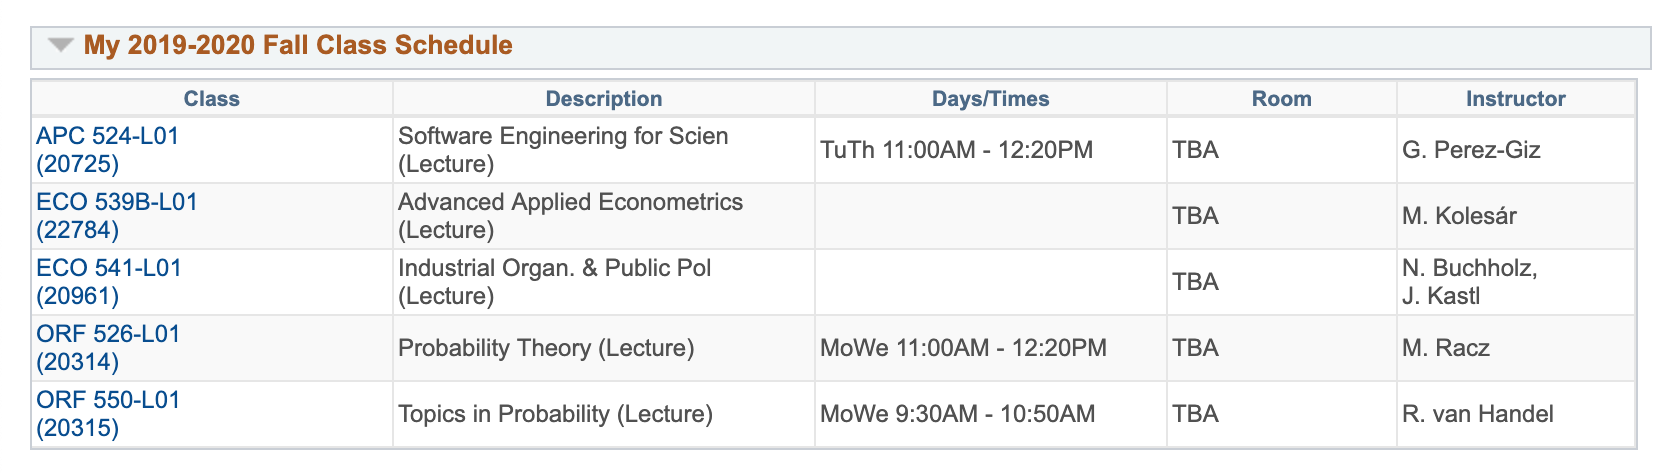
\includegraphics[width=1.2\textwidth]{schedule.png}
    }
    % \caption{Caption}
    \label{fig:my_label}
\end{figure}
\section{SDSC Summer Institute Summary}
Lecture materials and reference materials available at \url{https://github.com/sdsc/sdsc-summer-institute-2019} Below is a list of what I gained from attending. 

\begin{itemize}
    \item Reviewed how to use git
    \item Learned about best practices for submitting jobs to supercomputing systems (SLURM files, Singularity containers)
    \item Learned about hardware -- GPU vs. CPU, computing clusters
    \item Python for HPC -- using Dask to paralellize code locally and distributed on a network; using Numba to speedup code locally
    \item Performance tuning tips in C and Fortran
    \item Machine learning overview in R
    \item Intro to GPU Programming with Cuda
    \item Deep learning with neural networks and Keras in Python 
    \item Made short presentation about research  in lightning rounds
    \item Introduction to XSEDE supercomputing resources (which I have access to as an NSF honorable mention)
    \item Interest in applying econometrics to environmental data problems (discuss this more?)
\end{itemize}

\newpage
\section{Third year paper}
\subsection{Proposed timeline}
\noindent August 26 -- Research topic selected, submit to Bo an initial research proposal

\noindent August 30 -- Description of model, parameter of interest, general problem, preliminary assumptions (i.e. an introduction)

\noindent September 6 -- Annotated Bibliography 

\noindent September 13 -- Proposed methodology

\noindent September 25 -- Empirical example (simulations or data work) 

\noindent October 1 -- First draft done

\noindent Week of October 5 -- Present in student seminar 

\noindent October 28 -- Final draft done

\noindent November 4 -- Last day for submission
\subsection*{Idea \#1: Extend imperfect matching paper}

Here are some possible extensions I could imagine pursuing.  
\begin{enumerate}
    \item What if $\{y_{i\ell}\}$ does not contain the true match for some $i$?  Can we make our estimator robust to this possibility?
    \item Is there a bias/variance tradeoff for including/excluding observations with multiple matches in finite samples? Similarly, are there tradeoffs for other setting-specific variants, such as large $L_i$, imprecise $\hat{g}$, small proportion of observations with $L_i > 1$, or we can precisely estimate the probability of a correct match
    \item Can we construct informative bounds for $\theta_0$ by considering multiple configurations of matched data, or composite datapoints? 
\end{enumerate}





\subsection*{Idea \#2: Replicate  Aizer et al. (2016) with a fully Bayesian framework}

Bayesian methods are appealing as a tool to understand heterogeneous treatment effects, as well as propagate uncertainty from all stages of the analysis -- from censorship, multiple matches, missing data -- into confidence sets about $\theta$.  My hope in using Bayesian methods is to extract more information from observations that were dropped by Aizer et al. (2016) because they were missing variables (or female), and produce an example of how Bayesian methods can be used to address data challenges that appear frequently in applied microeconometrics.  

The first regression in the Aizer et al (2016) paper is:
\begin{equation} \log (\text{age at death})_{ifts} = \theta_0 + \theta_1 MP_f + \theta_2 X_{if} + \theta_3 Z_{st} + \theta_c + \theta_t + \epsilon_{if}
 \label{aer} \end{equation}
where the dependent variable is the natural log of the age at death for a given individual $i$ in family $f$ born in year $t$ in county $c$ (state $s$).  $MP_f$ is an indicator for whether the child's family received MP benefits, and $X$ is a vector of relevant family and characteristics.  $Z_{st}$ are state and year level controls, and $\theta_c$ and $\theta_t$ are county and cohort fixed effects.  The effect of the program $\theta_1$ is identified by comparing the average age at death of accepted boys to rejected boys within county and year of birth, conditional on other observables.

As discussed in Gelman et al. (2014), there are difficulties associated with both separate and pooled estimates of treatment effects. I would begin my analysis by estimating a normal hierarchical model with exchangeable parameters in place of (\ref{aer}). 

\end{document}
